	\section{Computational experiments}\label{section:experiments}
This section is devoted to studying the performance of \eqref{form:H-TSPHN} and \eqref{form:H-TSPN} formulations proposed in Section \ref{section:formulations}. In the first subsection, the procedure for generating the considered random instances is described. The second subsection details the experiments that have been conducted. The third subsection reports the results obtained in these experiments.

\subsection{Data generation}
%To generate the instances of our experiments, it is necessary that these instances verify the assumptions \ref{A1}-\ref{A4} stated in the Section \ref{section:description}. 

To generate the instances of our experiments, we assume  assumptions \ref{A1}-\ref{A4} stated in Section \ref{section:description}. The following proposition gives an upper bound for the number of balls that can be generated given an instance with $n=|\mathcal B|$ barriers:

%		\JP{	
	%		\begin{prop}
		%			Under the hypothesis that balls are \CV{not} visible among them, the maximum number of balls that can be considered in \TSPHN \ is $O(n^2)$.
		%		\end{prop}
	%		\begin{proof}
		%			The proof is based on the properties of the visibility graph $VG(\cal B)$ of the configuration of barriers in $\cal B$:  It is clear that the maximum number of balls coincides with the number of faces, $f_{VG(\cal B)}$, of $VG(\cal B)$.  Recall that the number of vertices in $\cal B$ is $n$. Next, by the Euler formula, the number of faces $f_{VG(\cal B)}$ is $2+E_{VG(\cal B)}-n$. Since $E_{VG(\cal B)}=O(n^2)$, it follows that $f_{VG(\cal B)}=O(n^2)$.
		%		\end{proof}
	%	}


\begin{prop}
	Under assumptions \ref{A1}-\ref{A4}, the maximum number of balls that can be considered in \TSPHN \ is $O(n^2)$.
\end{prop}
\begin{proof}
	The proof is based on the properties of the visibility graph $VG(\cal B)$ of the configuration of barriers in $\cal B$ \citep{mitchell_shortest_2017}:  It is clear that the maximum number of balls coincides with the number of faces, $f_{VG(\cal B)}$, of $VG(\cal B)$.  Recall that the number of vertices in $\cal B$ is $n$. Next, by the Euler formula the number of faces $f_{VG(\cal B)}$ is $2+E_{VG(\cal B)}-n$. Since $E_{VG(\cal B)}=O(n^2)$, it follows that $f_{VG(\cal B)}=O(n^2)$.
\end{proof}


The idea is to generate line segments located in general position without crossings and neighbourhoods that do not intersect with these line segments. The following procedure describes how to construct instances where the neighbourhoods are balls.

\begin{algorithm}[H]
	\caption{Generation of instances when the neighbourhoods are balls}
	\label{alg:Algorithm3}
	\SetKwInOut{Input}{Initialization}\SetKwInOut{Output}{output}
	
	\Input{Let $|\mathcal N|$ be the number of neighbourhoods to generate. Let $r_{\text{init}}=10$ be half of the initial length of the barriers.
		Set $\mathcal N = \{\}$; $points=\{\}$; $\mathcal B=\{\overline{(0, 0)(100, 0)}, \overline{(100, 0)(100, 100)}, \overline{(100, 100)(0, 100)}, \overline{(0, 100)(0, 0)}\}$.}
	% Set $LB=0$, $UB=+\infty$, $\bar z=z^0$.
	Generate $|\mathcal N|$ points uniformly distributed in the square $[0, 100]^2$ and include them in $points$. \\
	%\While{There does not exist a barrier that separates each pair of points}{
		\For{$P, P'\in points$}{
			\If{$\overline{PP'}\cap B=\emptyset,\;\forall B\in\mathcal B$}{
				Compute $\overrightarrow{d}=\overrightarrow{PP'}$.\\
				Compute $M = P + \frac 1 2 \overrightarrow{d}$.\\
				Compute the unitary vector $\overrightarrow{n_u}$ perpendicular to $\overrightarrow{d}$.\\
				Set $r = r_{\text{init}}$. \\
				Generate the barrier $B(r)=\overline{P_B^{+} P_B^{-}}$ where
				$P_B^{\pm}=M \pm r\overrightarrow{n_u}.$\\
				\While{$B(r)\cap B'\neq\emptyset$ for some $B'\in\mathcal B$}{
					Set $r := r / 2$. \\
					Generate the barrier $B(r)$.
				}
				
				Include $B(r)$ in $\mathcal B$.
				
				
			}
		}
		\For{$P\in points$}{
			Set $r_{\text{max}}=\min_{\{P_B\in B: B \in\mathcal B\}} d(P, P_B).$\\
			Generate a random $radii$ uniformly distributed in the interval $\left[\frac 1 2 r_{\text{max}}, r_{\text{max}}\right]$.\\
			Set the ball $N$ whose centre is $P$ and radii is $radii$. \\
			Include $N$ in $\mathcal N$.
		}
		%}
\end{algorithm}
The line segments instances are generated by randomly selecting two diametrically opposite points in the boundary of the balls instances obtained with Algorithm \ref{alg:Algorithm3}.
%	To generate the instances when the neighbourhoods are segments, we can take the balls built in the previous procedure and draw a random angle that determines which point and its diametrically opposite point are selected as the endpoints of the line segment.

% \textcolor{red}{Quizás evitar el uso $n$ sea adecuado para evitar confusiones}
\subsection{Configuration of the experiments}
Since no benchmark instances are available for this problem in the literature, we have generated five instances with a number of neighbourhoods $|\mathcal N|\in\{5, 10, 20, 30, 50, 80, 100\}$ of two typologies: balls and line segments. We have distinguished the cases with and without \sout{preprocessing the variables of} \CV{strengthening} the formulations, as explained in Section \ref{section:strengthening}, and we have reported the average results. 

The formulations were coded in Python 3.9.2 (\citet{g_van_rossum_guido_python_1995}) and solved in Gurobi 9.1.2 (\citet{gurobi_optimization_llc_gurobi_2022}) on an AMD® Epyc 7402p 8-core processor. A time limit of 1 hour was set in the experiments.

\subsection{Results of the experiments}
We report the results of our experiments in Table \ref{table:results}. The layout is organised in 5 blocks of columns. The first one describes the number of neighbourhoods $|\mathcal{N}|$, the second (neighbourhood) describes the typology of neighbourhood used in the experiment (Balls or Segments), the third one (strengthening)  informs whether the strengthening is being applied or not (True or False). The next three blocks include information  on the number of barriers ($|\mathcal{B}|$), the  gap at termination (Gap) defined as $Gap=(upper\, bound - lower\, bound)/lower\, bound$, and the computing time (Runtime). The block $|\mathcal{B}|$ indicates the minimum and maximum number of barriers considered in each of the instances for each fixed number $|\mathcal{N}|$ of neighbours. The block Gap contains three columns reporting the average (mean), minimum (min), and maximum (max) gaps of the ten instances considered for each combination of parameters. Analogously, the block Runtime also includes three columns reporting the average (mean), minimum (min) and maximum (max) computing time of the ten instances considered for each combination of parameters.
By rows, Table \ref{table:results} reports results for instances with a number of neigbourhoods $|\mathcal{N}|$ in the set $\{5,10,20,30,50,80,100\}$. For each value of $|\mathcal{N}|$  we report results for two typologies of neigbourhoods, namely Balls and Segments, without strengthening (False) and with strengthening (True).

Analysing the results in Table \ref{table:results}, first of all we observe that solving the problem considering balls as neighbourhoods is harder than considering segments. Next, we also observe that our formulation solves to optimality all instances for segments up to $|\mathcal{N}|=30$ with strengthening. In addition, both typologies of instances, up to $|\mathcal{N}|=50$, are almost solved by obtaining a small average gap. %and also almost all for balls leaving always a gap less than or equal to  1\%. 
We also observe that the use of strengthening helps in solving the instances since in those cases where they are not solved to optimality the gap and the runtime are reduced. The situation for $|\mathcal{N}|\in \{80,100\}$ is slightly different. For $|\mathcal{N}|=80$ and balls as neighbourhoods, the strengthening time takes more than an hour so that no results can be reported whereas without strengthening the formulations are always able to find solutions with average gaps of ($\le 0.6$) within one hour of computing time.  % For segments we see that the use of strengthening helps and the gaps are smaller within the time limit. 
Finally, for the case of $|\mathcal{N}|=100$ balls as neighbourhoods, none of the configurations with or without strengthening is capable to find a feasible solution in 3600 seconds. The behaviour is different for segments. In this case, both configurations provide feasible solutions. In the last case, the use of strengthening is rather heavy and consumes most of the 3600 seconds of computing time. This can be observed in the final gaps. The case without strengthening reports better gaps, as leaving more time to the solver to find better solutions, and the average gap is $0.53$ rather than $0.81$ for the case with strengthening.

%% Table generated by Excel2LaTeX from sheet 'Hoja1'
%\begin{table}[htbp]
%	\centering
%	\caption{Add caption}
%	\resizebox{\textwidth}{!}{
	%	\begin{tabular}{|c|c|c||cc|ccc|ccc|}
		%		\hline
		%		$\bm{|\mathcal N|}$ & \textbf{Typology} & \textbf{strengthening} & \multicolumn{2}{c|}{$\bm{|\mathcal B|}$} & \multicolumn{3}{c|}{\textbf{Gap}} & \multicolumn{3}{c|}{\textbf{Runtime}} \bigstrut[t]\\
		%		&       &       & \textbf{min} & \textbf{max} & \textbf{mean} & \textbf{min} & \textbf{max} & \textbf{mean} & \textbf{min} & \textbf{max} \bigstrut[b]\\
		%		\hline
		%		\hline
		%		\multirow{4}[4]{*}{5} & \multirow{2}[2]{*}{Ball} & False & 8     & 11    & 0     & 0     & 0     & 2.46  & 1.2   & 8.05 \bigstrut[t]\\
		%		&       & True  & 8     & 11    & 0     & 0     & 0     & 1.63  & 0.81  & 2.49 \bigstrut[b]\\
		%		\cline{2-11}          & \multirow{2}[2]{*}{Segment} & False & 8     & 11    & 0     & 0     & 0     & 1.35  & 0.82  & 2.52 \bigstrut[t]\\
		%		&       & True  & 8     & 11    & 0     & 0     & 0     & 1.09  & 0.79  & 1.41 \bigstrut[b]\\
		%		\hline
		%		\hline
		%		\multirow{4}[4]{*}{10} & \multirow{2}[2]{*}{Ball} & False & 15    & 21    & 0     & 0     & 0     & 13.43 & 7.85  & 27.68 \bigstrut[t]\\
		%		&       & True  & 15    & 21    & 0     & 0     & 0     & 6.22  & 3.61  & 11.85 \bigstrut[b]\\
		%		\cline{2-11}          & \multirow{2}[2]{*}{Segment} & False & 15    & 21    & 0     & 0     & 0     & 7.41  & 5.04  & 9.23 \bigstrut[t]\\
		%		&       & True  & 15    & 21    & 0     & 0     & 0     & 4.54  & 3.15  & 5.7 \bigstrut[b]\\
		%		\hline
		%		\hline
		%		\multirow{4}[4]{*}{20} & \multirow{2}[2]{*}{Ball} & False & 35    & 40    & 0     & 0     & 0     & 132.22 & 58.21 & 225.89 \bigstrut[t]\\
		%		&       & True  & 35    & 40    & 0     & 0     & 0     & 45.86 & 20.32 & 104.49 \bigstrut[b]\\
		%		\cline{2-11}          & \multirow{2}[2]{*}{Segment} & False & 35    & 40    & 0     & 0     & 0     & 97.25 & 40.06 & 166.67 \bigstrut[t]\\
		%		&       & True  & 35    & 40    & 0     & 0     & 0     & 38.47 & 15.77 & 66.05 \bigstrut[b]\\
		%		\hline
		%		\hline
		%		\multirow{4}[4]{*}{30} & \multirow{2}[2]{*}{Ball} & False & 49    & 60    & 0     & 0     & 0     & 373.32 & 246.51 & 639.97 \bigstrut[t]\\
		%		&       & True  & 49    & 60    & 0     & 0     & 0     & 127.15 & 53.08 & 219.85 \bigstrut[b]\\
		%		\cline{2-11}          & \multirow{2}[2]{*}{Segment} & False & 49    & 60    & 0     & 0     & 0     & 414.11 & 156.76 & 979.68 \bigstrut[t]\\
		%		&       & True  & 49    & 60    & 0     & 0     & 0     & 112.68 & 50.66 & 182.82 \bigstrut[b]\\
		%		\hline
		%		\hline
		%		\multirow{4}[4]{*}{50} & \multirow{2}[2]{*}{Ball} & False & 79    & 91    & 0     & 0     & 0.01  & 1634.35 & 603.48 & 3605.13 \bigstrut[t]\\
		%		&       & True  & 79    & 91    & 0     & 0     & 0     & 553.93 & 181.13 & 1599.18 \bigstrut[b]\\
		%		\cline{2-11}          & \multirow{2}[2]{*}{Segment} & False & 79    & 91    & 0     & 0     & 0.01  & 1618.95 & 855.65 & 3604.93 \bigstrut[t]\\
		%		&       & True  & 79    & 91    & 0     & 0     & 0     & 523.08 & 152.08 & 1548.64 \bigstrut[b]\\
		%		\hline
		%		\hline
		%		\multirow{4}[4]{*}{80} & \multirow{2}[2]{*}{Ball} & False & 125   & 145   & -     & -     & -     & -     & -     & - \bigstrut[t]\\
		%		&       & True  & 125   & 145   & 0.01  & 0     & 0.02  & 3110.68 & 1976.01 & 3601.13 \bigstrut[b]\\
		%		\cline{2-11}          & \multirow{2}[2]{*}{Segment} & False & 125   & 145   & -     & -     & -     & -     & -     & - \bigstrut[t]\\
		%		&       & True  & 125   & 145   & 0.01  & 0     & 0.03  & 2835.09 & 1663.53 & 3601.26 \bigstrut[b]\\
		%		\hline
		%	\end{tabular}}%
%	\label{tab:addlabel}%
%\end{table}%

% Table generated by Excel2LaTeX from sheet 'Hoja1'
\begin{table}[htbp]
	\centering
	\caption{Table of computational results obtained with the formulation \eqref{form:H-TSPHN}}
	\resizebox{\textwidth}{!}{
		\begin{tabular}{|c|c|c||cc|ccc|ccc|}
			\hline
			$\bm{|\mathcal N|}$ & \textbf{neighbourhood} & \textbf{strengthening} & \multicolumn{2}{c|}{$\bm{|\mathcal B|}$} & \multicolumn{3}{c|}{\textbf{Gap}} & \multicolumn{3}{c|}{\textbf{Runtime}} \bigstrut[t]\\
			&       &       & \textbf{min} & \textbf{max} & \textbf{mean} & \textbf{min} & \textbf{max} & \textbf{mean} & \textbf{min} & \textbf{max} \bigstrut[b]\\
			\hline
			\hline
			\multirow{4}[4]{*}{5} & \multirow{2}[2]{*}{Ball} & False & \multirow{4}[4]{*}{8} & \multirow{4}[4]{*}{11} & 0.05  & 0     & 0.55  & 371.84 & 2.96  & 3600 \bigstrut[t]\\
			&       & True  &       &       & 0     & 0     & 0     & 3.46  & 1.4   & 13 \bigstrut[b]\\
			\cline{2-3}\cline{6-11}          & \multirow{2}[2]{*}{Segment} & False &       &       & 0.08  & 0     & 0.49  & 1085.48 & 0.68  & 3600 \bigstrut[t]\\
			&       & True  &       &       & 0     & 0     & 0     & 1.44  & 0.6   & 2.46 \bigstrut[b]\\
			\hline
			\hline
			\multirow{4}[4]{*}{10} & \multirow{2}[2]{*}{Ball} & False & \multirow{4}[4]{*}{15} & \multirow{4}[4]{*}{21} & 0.17  & 0     & 0.86  & 998.71 & 59.09 & 3600 \bigstrut[t]\\
			&       & True  &       &       & 0     & 0     & 0     & 36.66 & 10.72 & 87.29 \bigstrut[b]\\
			\cline{2-3}\cline{6-11}          & \multirow{2}[2]{*}{Segment} & False &       &       & 0.33  & 0     & 0.86  & 1460.31 & 16.78 & 3600 \bigstrut[t]\\
			&       & True  &       &       & 0     & 0     & 0     & 8.53  & 2.66  & 12.25 \bigstrut[b]\\
			\hline
			\hline
			\multirow{4}[4]{*}{20} & \multirow{2}[2]{*}{Ball} & False & \multirow{4}[4]{*}{35} & \multirow{4}[4]{*}{40} & 0.06  & 0.02  & 0.1   & 3600  & 3600  & 3600 \bigstrut[t]\\
			&       & True  &       &       & 0     & 0     & 0.01  & 1424.85 & 140.54 & 3600 \bigstrut[b]\\
			\cline{2-3}\cline{6-11}          & \multirow{2}[2]{*}{Segment} & False &       &       & 0     & 0     & 0.02  & 1430.13 & 166.89 & 3600 \bigstrut[t]\\
			&       & True  &       &       & 0     & 0     & 0     & 198.9 & 30.75 & 426.55 \bigstrut[b]\\
			\hline
			\hline
			\multirow{4}[4]{*}{30} & \multirow{2}[2]{*}{Ball} & False & \multirow{4}[4]{*}{49} & \multirow{4}[4]{*}{60} & 0.12  & 0     & 0.93  & 3566.2 & 3246.53 & 3600 \bigstrut[t]\\
			&       & True  &       &       & 0     & 0     & 0.02  & 2146.17 & 314.65 & 3600 \bigstrut[b]\\
			\cline{2-3}\cline{6-11}          & \multirow{2}[2]{*}{Segment} & False &       &       & 0     & 0     & 0.01  & 2119.06 & 315.56 & 3600 \bigstrut[t]\\
			&       & True  &       &       & 0     & 0     & 0     & 1140.02 & 353.73 & 3209.94 \bigstrut[b]\\
			\hline
			\hline
			\multirow{4}[4]{*}{50} & \multirow{2}[2]{*}{Ball} & False & \multirow{4}[4]{*}{79} & \multirow{4}[4]{*}{91} & 0.09  & 0.02  & 0.19  & 3600  & 3600  & 3600 \bigstrut[t]\\
			&       & True  &       &       & 0.08  & 0.01  & 0.21  & 3600  & 3600  & 3600 \bigstrut[b]\\
			\cline{2-3}\cline{6-11}          & \multirow{2}[2]{*}{Segment} & False &       &       & 0.02  & 0.01  & 0.09  & 3600  & 3600  & 3600 \bigstrut[t]\\
			&       & True  &       &       & 0.02  & 0     & 0.1   & 2956.24 & 2053.62 & 3600 \bigstrut[b]\\
			\hline
			\hline
			\multirow{4}[4]{*}{80} & \multirow{2}[2]{*}{Ball} & False & \multirow{4}[4]{*}{125} & \multirow{4}[4]{*}{145} & 0.6   & 0.42  & 0.79  & 3600  & 3600  & 3600 \bigstrut[t]\\
			&       & True  &       &       & -     & -     & -     & -     & -     & - \bigstrut[b]\\
			\cline{2-3}\cline{6-11}          & \multirow{2}[2]{*}{Segment} & False &       &       & 0.16  & 0.03  & 0.62  & 3600  & 3600  & 3600 \bigstrut[t]\\
			&       & True  &       &       & 0.61  & 0.01  & 1     & 3600  & 3600  & 3600 \bigstrut[b]\\
			\hline
			\hline
			\multirow{4}[4]{*}{100} & \multirow{2}[2]{*}{Ball} & False & \multirow{4}[4]{*}{156} & \multirow{4}[4]{*}{178} & -     & -     & -     & -     & -     & - \bigstrut[t]\\
			&       & True  &       &       & -     & -     & -     & -     & -     & - \bigstrut[b]\\
			\cline{6-11}          & \multirow{2}[2]{*}{Segment} & False &       &       & 0.53  & 0.02  & 0.99  & 3600  & 3600  & 3600 \bigstrut[t]\\
			&       & True  &       &       & 0.81  & 0.5   & 1     & 3600  & 3600  & 3600 \bigstrut[b]\\
			\hline
	\end{tabular}}%
	\label{table:results}%
\end{table}%

The same behaviour is also observed in Figure 9. The left subfigure reports the boxplot diagram for the experiments with segments as neighbourhoods, whereas the right one reports the boxplot diagram for balls as neighbourhoods. We see that strengthening always helps since the corresponding boxes are below those without strengthening, whenever the problems are solved well. Moreover,  we also observe in those cases where the model solves the instances  $|\mathcal{N}|\le 50$, that the problem with balls is harder than with segments since the boxes in the left subfigure are below the ones in the right subfigure.






% \DeclareUnicodeCharacter{2212}{−}
% \usepgfplotslibrary{groupplots}
\usetikzlibrary{patterns,shapes.arrows}
\pgfplotsset{compat=newest}

\definecolor{darkslategray38}{RGB}{38,38,38}
\definecolor{darkslategray76}{RGB}{76,76,76}
\definecolor{lavender234234242}{RGB}{234,234,242}
\definecolor{peru20313699}{RGB}{203,136,99}
\definecolor{steelblue88116163}{RGB}{88,116,163}

\begin{figure}[h!]
    \centering
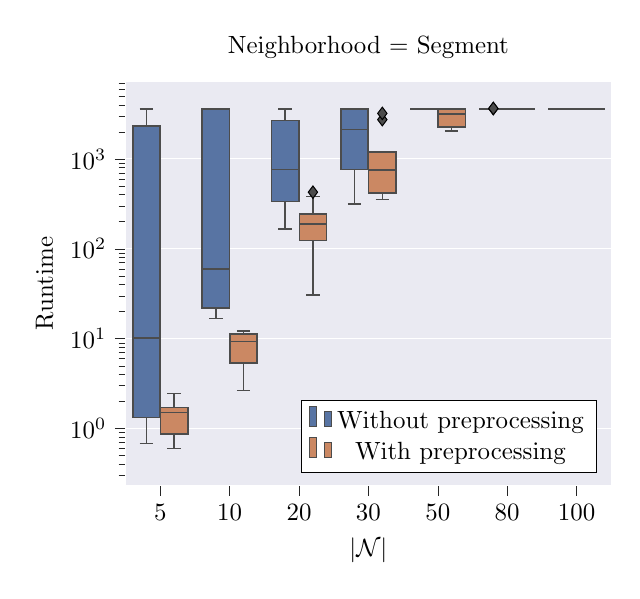
\begin{tikzpicture}[scale=0.9]

\definecolor{color0}{rgb}{0.917647058823529,0.917647058823529,0.949019607843137}
\definecolor{color1}{rgb}{0.347058823529412,0.458823529411765,0.641176470588235}
\definecolor{color2}{rgb}{0.798529411764706,0.536764705882353,0.389705882352941}

\begin{axis}[
axis background/.style={fill=color0},
axis line style={white},
tick align=outside,
title={Neighborhood = Segment},
x grid style={white},
xtick pos = left,
ytick pos = left,
xlabel={$|\mathcal N|$},
% xmajorticks=false,
xmin=-0.5, xmax=6.5,
xtick style={color=white!15!black},
xtick={0,1,2,3,4,5,6},
xticklabels={5, 10, 20, 30, 50, 80, 100},
y grid style={white},
ylabel={Runtime},
ymajorgrids,
% ymajorticks=false,
ymin=-0.05, ymax= 7200,
log basis y={10},
ymode = log,
ytick style={color=white!15!black},
%ytick={-0.2,0,0.2,0.4,0.6,0.8,1,1.2},
%yticklabels={−0.2,0.0,0.2,0.4,0.6,0.8,1.0,1.2},
legend pos = south east
]
\path [draw=darkslategray76, fill=steelblue88116163, semithick]
(axis cs:-0.396,1.32029229402542)
--(axis cs:-0.004,1.32029229402542)
--(axis cs:-0.004,2321.5214869976)
--(axis cs:-0.396,2321.5214869976)
--(axis cs:-0.396,1.32029229402542)
--cycle;
\path [draw=darkslategray76, fill=peru20313699, semithick]
(axis cs:0.004,0.867011845111847)
--(axis cs:0.396,0.867011845111847)
--(axis cs:0.396,1.71693199872971)
--(axis cs:0.004,1.71693199872971)
--(axis cs:0.004,0.867011845111847)
--cycle;
\path [draw=darkslategray76, fill=steelblue88116163, semithick]
(axis cs:0.604,22.0478292107582)
--(axis cs:0.996,22.0478292107582)
--(axis cs:0.996,3600.1058292985)
--(axis cs:0.604,3600.1058292985)
--(axis cs:0.604,22.0478292107582)
--cycle;
\path [draw=darkslategray76, fill=peru20313699, semithick]
(axis cs:1.004,5.35795325040817)
--(axis cs:1.396,5.35795325040817)
--(axis cs:1.396,11.317633330822)
--(axis cs:1.004,11.317633330822)
--(axis cs:1.004,5.35795325040817)
--cycle;
\path [draw=darkslategray76, fill=steelblue88116163, semithick]
(axis cs:1.604,336.735125482082)
--(axis cs:1.996,336.735125482082)
--(axis cs:1.996,2661.89892309904)
--(axis cs:1.604,2661.89892309904)
--(axis cs:1.604,336.735125482082)
--cycle;
\path [draw=darkslategray76, fill=peru20313699, semithick]
(axis cs:2.004,124.047738432884)
--(axis cs:2.396,124.047738432884)
--(axis cs:2.396,243.347989618778)
--(axis cs:2.004,243.347989618778)
--(axis cs:2.004,124.047738432884)
--cycle;
\path [draw=darkslategray76, fill=steelblue88116163, semithick]
(axis cs:2.604,758.177148163319)
--(axis cs:2.996,758.177148163319)
--(axis cs:2.996,3601.57422971725)
--(axis cs:2.604,3601.57422971725)
--(axis cs:2.604,758.177148163319)
--cycle;
\path [draw=darkslategray76, fill=peru20313699, semithick]
(axis cs:3.004,415.898770868778)
--(axis cs:3.396,415.898770868778)
--(axis cs:3.396,1199.34626537561)
--(axis cs:3.004,1199.34626537561)
--(axis cs:3.004,415.898770868778)
--cycle;
\path [draw=darkslategray76, fill=steelblue88116163, semithick]
(axis cs:3.604,3601.05894333124)
--(axis cs:3.996,3601.05894333124)
--(axis cs:3.996,3606.46183502674)
--(axis cs:3.604,3606.46183502674)
--(axis cs:3.604,3601.05894333124)
--cycle;
\path [draw=darkslategray76, fill=peru20313699, semithick]
(axis cs:4.004,2274.12813621759)
--(axis cs:4.396,2274.12813621759)
--(axis cs:4.396,3604.64131337404)
--(axis cs:4.004,3604.64131337404)
--(axis cs:4.004,2274.12813621759)
--cycle;
\path [draw=darkslategray76, fill=steelblue88116163, semithick]
(axis cs:4.604,3603.31649148464)
--(axis cs:4.996,3603.31649148464)
--(axis cs:4.996,3606.0530809164)
--(axis cs:4.604,3606.0530809164)
--(axis cs:4.604,3603.31649148464)
--cycle;
\path [draw=darkslategray76, fill=peru20313699, semithick]
(axis cs:5.004,3602.73281055689)
--(axis cs:5.396,3602.73281055689)
--(axis cs:5.396,3617.00508999825)
--(axis cs:5.004,3617.00508999825)
--(axis cs:5.004,3602.73281055689)
--cycle;
\path [draw=darkslategray76, fill=steelblue88116163, semithick]
(axis cs:5.604,3604.5290222168)
--(axis cs:5.996,3604.5290222168)
--(axis cs:5.996,3639.30546808243)
--(axis cs:5.604,3639.30546808243)
--(axis cs:5.604,3604.5290222168)
--cycle;
\path [draw=darkslategray76, fill=peru20313699, semithick]
(axis cs:6.004,3603.62441074848)
--(axis cs:6.396,3603.62441074848)
--(axis cs:6.396,3604.991119802)
--(axis cs:6.004,3604.991119802)
--(axis cs:6.004,3603.62441074848)
--cycle;
\path [draw=darkslategray76, fill=steelblue88116163, semithick]
(axis cs:6.604,3613.56903254986)
--(axis cs:6.996,3613.56903254986)
--(axis cs:6.996,3668.42798751593)
--(axis cs:6.604,3668.42798751593)
--(axis cs:6.604,3613.56903254986)
--cycle;
\path [draw=darkslategray76, fill=peru20313699, semithick]
(axis cs:7.004,3604.49900507927)
--(axis cs:7.396,3604.49900507927)
--(axis cs:7.396,3605.37177205086)
--(axis cs:7.004,3605.37177205086)
--(axis cs:7.004,3604.49900507927)
--cycle;
\draw[draw=darkslategray76,fill=steelblue88116163,line width=0.3pt] (axis cs:0,0) rectangle (axis cs:0,0);
\addlegendimage{ybar,ybar legend,draw=darkslategray76,fill=steelblue88116163,line width=0.3pt}
\addlegendentry{Without preprocessing}

\draw[draw=darkslategray76,fill=peru20313699,line width=0.3pt] (axis cs:0,0) rectangle (axis cs:0,0);
\addlegendimage{ybar,ybar legend,draw=darkslategray76,fill=peru20313699,line width=0.3pt}
\addlegendentry{With preprocessing}

\addplot [semithick, darkslategray76]
table {%
	-0.2 1.32029229402542
	-0.2 0.679740905761719
};
\addplot [semithick, darkslategray76]
table {%
	-0.2 2321.5214869976
	-0.2 3600.04041099548
};
\addplot [semithick, darkslategray76]
table {%
	-0.298 0.679740905761719
	-0.102 0.679740905761719
};
\addplot [semithick, darkslategray76]
table {%
	-0.298 3600.04041099548
	-0.102 3600.04041099548
};
\addplot [semithick, darkslategray76]
table {%
	0.2 0.867011845111847
	0.2 0.598104000091553
};
\addplot [semithick, darkslategray76]
table {%
	0.2 1.71693199872971
	0.2 2.45890307426453
};
\addplot [semithick, darkslategray76]
table {%
	0.102 0.598104000091553
	0.298 0.598104000091553
};
\addplot [semithick, darkslategray76]
table {%
	0.102 2.45890307426453
	0.298 2.45890307426453
};
\addplot [semithick, darkslategray76]
table {%
	0.8 22.0478292107582
	0.8 16.7804238796234
};
\addplot [semithick, darkslategray76]
table {%
	0.8 3600.1058292985
	0.8 3600.14186501503
};
\addplot [semithick, darkslategray76]
table {%
	0.702 16.7804238796234
	0.898 16.7804238796234
};
\addplot [semithick, darkslategray76]
table {%
	0.702 3600.14186501503
	0.898 3600.14186501503
};
\addplot [semithick, darkslategray76]
table {%
	1.2 5.35795325040817
	1.2 2.66339802742004
};
\addplot [semithick, darkslategray76]
table {%
	1.2 11.317633330822
	1.2 12.2503089904785
};
\addplot [semithick, darkslategray76]
table {%
	1.102 2.66339802742004
	1.298 2.66339802742004
};
\addplot [semithick, darkslategray76]
table {%
	1.102 12.2503089904785
	1.298 12.2503089904785
};
\addplot [semithick, darkslategray76]
table {%
	1.8 336.735125482082
	1.8 166.894387960434
};
\addplot [semithick, darkslategray76]
table {%
	1.8 2661.89892309904
	1.8 3600.55163097382
};
\addplot [semithick, darkslategray76]
table {%
	1.702 166.894387960434
	1.898 166.894387960434
};
\addplot [semithick, darkslategray76]
table {%
	1.702 3600.55163097382
	1.898 3600.55163097382
};
\addplot [semithick, darkslategray76]
table {%
	2.2 124.047738432884
	2.2 30.748733997345
};
\addplot [semithick, darkslategray76]
table {%
	2.2 243.347989618778
	2.2 380.830942869186
};
\addplot [semithick, darkslategray76]
table {%
	2.102 30.748733997345
	2.298 30.748733997345
};
\addplot [semithick, darkslategray76]
table {%
	2.102 380.830942869186
	2.298 380.830942869186
};
\addplot [black, mark=diamond*, mark size=2.5, mark options={solid,fill=darkslategray76}, only marks]
table {%
	2.2 426.554292917252
};
\addplot [semithick, darkslategray76]
table {%
	2.8 758.177148163319
	2.8 315.556146144867
};
\addplot [semithick, darkslategray76]
table {%
	2.8 3601.57422971725
	2.8 3601.94508290291
};
\addplot [semithick, darkslategray76]
table {%
	2.702 315.556146144867
	2.898 315.556146144867
};
\addplot [semithick, darkslategray76]
table {%
	2.702 3601.94508290291
	2.898 3601.94508290291
};
\addplot [semithick, darkslategray76]
table {%
	3.2 415.898770868778
	3.2 353.725795984268
};
\addplot [semithick, darkslategray76]
table {%
	3.2 1199.34626537561
	3.2 1215.04742217064
};
\addplot [semithick, darkslategray76]
table {%
	3.102 353.725795984268
	3.298 353.725795984268
};
\addplot [semithick, darkslategray76]
table {%
	3.102 1215.04742217064
	3.298 1215.04742217064
};
\addplot [black, mark=diamond*, mark size=2.5, mark options={solid,fill=darkslategray76}, only marks]
table {%
	3.2 2735.75876998901
	3.2 3209.93583416939
};
\addplot [semithick, darkslategray76]
table {%
	3.8 3601.05894333124
	3.8 3600.85991501808
};
\addplot [semithick, darkslategray76]
table {%
	3.8 3606.46183502674
	3.8 3607.48930191994
};
\addplot [semithick, darkslategray76]
table {%
	3.702 3600.85991501808
	3.898 3600.85991501808
};
\addplot [semithick, darkslategray76]
table {%
	3.702 3607.48930191994
	3.898 3607.48930191994
};
\addplot [semithick, darkslategray76]
table {%
	4.2 2274.12813621759
	4.2 2053.62032914162
};
\addplot [semithick, darkslategray76]
table {%
	4.2 3604.64131337404
	4.2 3607.03867697716
};
\addplot [semithick, darkslategray76]
table {%
	4.102 2053.62032914162
	4.298 2053.62032914162
};
\addplot [semithick, darkslategray76]
table {%
	4.102 3607.03867697716
	4.298 3607.03867697716
};
\addplot [semithick, darkslategray76]
table {%
	4.8 3603.31649148464
	4.8 3602.91880893707
};
\addplot [semithick, darkslategray76]
table {%
	4.8 3606.0530809164
	4.8 3606.30187892914
};
\addplot [semithick, darkslategray76]
table {%
	4.702 3602.91880893707
	4.898 3602.91880893707
};
\addplot [semithick, darkslategray76]
table {%
	4.702 3606.30187892914
	4.898 3606.30187892914
};
\addplot [black, mark=diamond*, mark size=2.5, mark options={solid,fill=darkslategray76}, only marks]
table {%
	4.8 3625.4150249958
	4.8 3645.45013308525
};
\addplot [semithick, darkslategray76]
table {%
	5.2 3602.73281055689
	5.2 3602.33397316933
};
\addplot [semithick, darkslategray76]
table {%
	5.2 3617.00508999825
	5.2 3624.0230820179
};
\addplot [semithick, darkslategray76]
table {%
	5.102 3602.33397316933
	5.298 3602.33397316933
};
\addplot [semithick, darkslategray76]
table {%
	5.102 3624.0230820179
	5.298 3624.0230820179
};
\addplot [semithick, darkslategray76]
table {%
	5.8 3604.5290222168
	5.8 3604.30805683136
};
\addplot [semithick, darkslategray76]
table {%
	5.8 3639.30546808243
	5.8 3645.38289093971
};
\addplot [semithick, darkslategray76]
table {%
	5.702 3604.30805683136
	5.898 3604.30805683136
};
\addplot [semithick, darkslategray76]
table {%
	5.702 3645.38289093971
	5.898 3645.38289093971
};
\addplot [semithick, darkslategray76]
table {%
	6.2 3603.62441074848
	6.2 3603.08717489243
};
\addplot [semithick, darkslategray76]
table {%
	6.2 3604.991119802
	6.2 3605.26269197464
};
\addplot [semithick, darkslategray76]
table {%
	6.102 3603.08717489243
	6.298 3603.08717489243
};
\addplot [semithick, darkslategray76]
table {%
	6.102 3605.26269197464
	6.298 3605.26269197464
};
\addplot [semithick, darkslategray76]
table {%
	6.8 3613.56903254986
	6.8 3605.69076514244
};
\addplot [semithick, darkslategray76]
table {%
	6.8 3668.42798751593
	6.8 3675.8382871151
};
\addplot [semithick, darkslategray76]
table {%
	6.702 3605.69076514244
	6.898 3605.69076514244
};
\addplot [semithick, darkslategray76]
table {%
	6.702 3675.8382871151
	6.898 3675.8382871151
};
\addplot [semithick, darkslategray76]
table {%
	7.2 3604.49900507927
	7.2 3603.45564484596
};
\addplot [semithick, darkslategray76]
table {%
	7.2 3605.37177205086
	7.2 3605.82377719879
};
\addplot [semithick, darkslategray76]
table {%
	7.102 3603.45564484596
	7.298 3603.45564484596
};
\addplot [semithick, darkslategray76]
table {%
	7.102 3605.82377719879
	7.298 3605.82377719879
};
\addplot [black, mark=diamond*, mark size=2.5, mark options={solid,fill=darkslategray76}, only marks]
table {%
	7.2 3658.00065898895
};
\addplot [semithick, darkslategray76]
table {%
	-0.396 10.1803375482559
	-0.004 10.1803375482559
};
\addplot [semithick, darkslategray76]
table {%
	0.004 1.51285195350647
	0.396 1.51285195350647
};
\addplot [semithick, darkslategray76]
table {%
	0.604 59.596302986145
	0.996 59.596302986145
};
\addplot [semithick, darkslategray76]
table {%
	1.004 9.26608741283417
	1.396 9.26608741283417
};
\addplot [semithick, darkslategray76]
table {%
	1.604 761.183493494987
	1.996 761.183493494987
};
\addplot [semithick, darkslategray76]
table {%
	2.004 188.488757133484
	2.396 188.488757133484
};
\addplot [semithick, darkslategray76]
table {%
	2.604 2137.81448185444
	2.996 2137.81448185444
};
\addplot [semithick, darkslategray76]
table {%
	3.004 755.287425994873
	3.396 755.287425994873
};
\addplot [semithick, darkslategray76]
table {%
	3.604 3606.29241991043
	3.996 3606.29241991043
};
\addplot [semithick, darkslategray76]
table {%
	4.004 3148.22736597061
	4.396 3148.22736597061
};
\addplot [semithick, darkslategray76]
table {%
	4.604 3603.71865308285
	4.996 3603.71865308285
};
\addplot [semithick, darkslategray76]
table {%
	5.004 3604.7077203989
	5.396 3604.7077203989
};
\addplot [semithick, darkslategray76]
table {%
	5.604 3606.53671908379
	5.996 3606.53671908379
};
\addplot [semithick, darkslategray76]
table {%
	6.004 3604.49580192566
	6.396 3604.49580192566
};
\addplot [semithick, darkslategray76]
table {%
	6.604 3661.83730447292
	6.996 3661.83730447292
};
\addplot [semithick, darkslategray76]
table {%
	7.004 3604.87411022186
	7.396 3604.87411022186
};
\end{axis}

\end{tikzpicture}
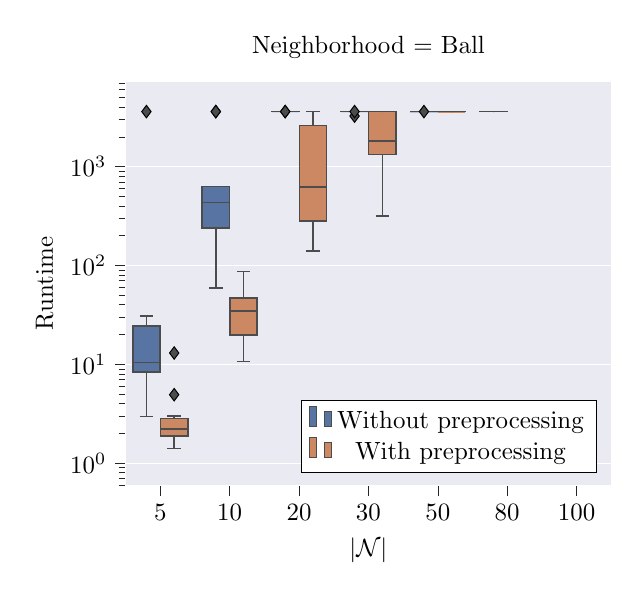
\begin{tikzpicture}[scale=0.9]

\definecolor{color0}{rgb}{0.917647058823529,0.917647058823529,0.949019607843137}
\definecolor{color1}{rgb}{0.347058823529412,0.458823529411765,0.641176470588235}
\definecolor{color2}{rgb}{0.798529411764706,0.536764705882353,0.389705882352941}

\begin{axis}[
axis background/.style={fill=color0},
axis line style={white},
tick align=outside,
title={Neighborhood = Ball},
x grid style={white},
xtick pos = left,
ytick pos = left,
xlabel={$|\mathcal N|$},
% xmajorticks=false,
xmin=-0.5, xmax=6.5,
xtick style={color=white!15!black},
xtick={0,1,2,3,4,5,6},
xticklabels={5, 10, 20, 30, 50, 80, 100},
y grid style={white},
ylabel={Runtime},
ymajorgrids,
% ymajorticks=false,
ymin=-0.05, ymax= 7200,
log basis y={10},
ymode = log,
ytick style={color=white!15!black},
%ytick={-0.2,0,0.2,0.4,0.6,0.8,1,1.2},
%yticklabels={−0.2,0.0,0.2,0.4,0.6,0.8,1.0,1.2},
legend pos = south east
]
\path [draw=darkslategray76, fill=steelblue88116163, semithick]
(axis cs:-0.396,8.35419070720673)
--(axis cs:-0.004,8.35419070720673)
--(axis cs:-0.004,24.3694642186165)
--(axis cs:-0.396,24.3694642186165)
--(axis cs:-0.396,8.35419070720673)
--cycle;
\path [draw=darkslategray76, fill=peru20313699, semithick]
(axis cs:0.004,1.88320851325989)
--(axis cs:0.396,1.88320851325989)
--(axis cs:0.396,2.84040707349777)
--(axis cs:0.004,2.84040707349777)
--(axis cs:0.004,1.88320851325989)
--cycle;
\path [draw=darkslategray76, fill=steelblue88116163, semithick]
(axis cs:0.604,240.028206408024)
--(axis cs:0.996,240.028206408024)
--(axis cs:0.996,626.305102109909)
--(axis cs:0.604,626.305102109909)
--(axis cs:0.604,240.028206408024)
--cycle;
\path [draw=darkslategray76, fill=peru20313699, semithick]
(axis cs:1.004,19.6992551088333)
--(axis cs:1.396,19.6992551088333)
--(axis cs:1.396,47.0685350894928)
--(axis cs:1.004,47.0685350894928)
--(axis cs:1.004,19.6992551088333)
--cycle;
\path [draw=darkslategray76, fill=steelblue88116163, semithick]
(axis cs:1.604,3600.64035725594)
--(axis cs:1.996,3600.64035725594)
--(axis cs:1.996,3600.77081692219)
--(axis cs:1.604,3600.77081692219)
--(axis cs:1.604,3600.64035725594)
--cycle;
\path [draw=darkslategray76, fill=peru20313699, semithick]
(axis cs:2.004,281.493759214878)
--(axis cs:2.396,281.493759214878)
--(axis cs:2.396,2610.16294920444)
--(axis cs:2.004,2610.16294920444)
--(axis cs:2.004,281.493759214878)
--cycle;
\path [draw=darkslategray76, fill=steelblue88116163, semithick]
(axis cs:2.604,3601.56696248055)
--(axis cs:2.996,3601.56696248055)
--(axis cs:2.996,3601.82251447439)
--(axis cs:2.604,3601.82251447439)
--(axis cs:2.604,3601.56696248055)
--cycle;
\path [draw=darkslategray76, fill=peru20313699, semithick]
(axis cs:3.004,1318.59078878164)
--(axis cs:3.396,1318.59078878164)
--(axis cs:3.396,3600.86907690764)
--(axis cs:3.004,3600.86907690764)
--(axis cs:3.004,1318.59078878164)
--cycle;
\path [draw=darkslategray76, fill=steelblue88116163, semithick]
(axis cs:3.604,3606.05540072918)
--(axis cs:3.996,3606.05540072918)
--(axis cs:3.996,3607.22088718414)
--(axis cs:3.604,3607.22088718414)
--(axis cs:3.604,3606.05540072918)
--cycle;
\path [draw=darkslategray76, fill=peru20313699, semithick]
(axis cs:4.004,3601.0776720047)
--(axis cs:4.396,3601.0776720047)
--(axis cs:4.396,3606.17869776487)
--(axis cs:4.004,3606.17869776487)
--(axis cs:4.004,3601.0776720047)
--cycle;
\path [draw=darkslategray76, fill=steelblue88116163, semithick]
(axis cs:4.604,3603.55773746967)
--(axis cs:4.996,3603.55773746967)
--(axis cs:4.996,3624.90419363976)
--(axis cs:4.604,3624.90419363976)
--(axis cs:4.604,3603.55773746967)
--cycle;
\draw[draw=darkslategray76,fill=steelblue88116163,line width=0.3pt] (axis cs:0,0) rectangle (axis cs:0,0);
\addlegendimage{ybar,ybar legend,draw=darkslategray76,fill=steelblue88116163,line width=0.3pt}
\addlegendentry{Without preprocessing}

\draw[draw=darkslategray76,fill=peru20313699,line width=0.3pt] (axis cs:0,0) rectangle (axis cs:0,0);
\addlegendimage{ybar,ybar legend,draw=darkslategray76,fill=peru20313699,line width=0.3pt}
\addlegendentry{With preprocessing}

\addplot [semithick, darkslategray76]
table {%
	-0.2 8.35419070720673
	-0.2 2.95881795883179
};
\addplot [semithick, darkslategray76]
table {%
	-0.2 24.3694642186165
	-0.2 30.9444210529327
};
\addplot [semithick, darkslategray76]
table {%
	-0.298 2.95881795883179
	-0.102 2.95881795883179
};
\addplot [semithick, darkslategray76]
table {%
	-0.298 30.9444210529327
	-0.102 30.9444210529327
};
\addplot [black, mark=diamond*, mark size=2.5, mark options={solid,fill=darkslategray76}, only marks]
table {%
	-0.2 3600.03402090073
};
\addplot [semithick, darkslategray76]
table {%
	0.2 1.88320851325989
	0.2 1.39969992637634
};
\addplot [semithick, darkslategray76]
table {%
	0.2 2.84040707349777
	0.2 2.98832607269287
};
\addplot [semithick, darkslategray76]
table {%
	0.102 1.39969992637634
	0.298 1.39969992637634
};
\addplot [semithick, darkslategray76]
table {%
	0.102 2.98832607269287
	0.298 2.98832607269287
};
\addplot [black, mark=diamond*, mark size=2.5, mark options={solid,fill=darkslategray76}, only marks]
table {%
	0.2 12.9982089996338
	0.2 4.92047095298767
};
\addplot [semithick, darkslategray76]
table {%
	0.8 240.028206408024
	0.8 59.0895512104034
};
\addplot [semithick, darkslategray76]
table {%
	0.8 626.305102109909
	0.8 628.835431814194
};
\addplot [semithick, darkslategray76]
table {%
	0.702 59.0895512104034
	0.898 59.0895512104034
};
\addplot [semithick, darkslategray76]
table {%
	0.702 628.835431814194
	0.898 628.835431814194
};
\addplot [black, mark=diamond*, mark size=2.5, mark options={solid,fill=darkslategray76}, only marks]
table {%
	0.8 3600.14500808716
	0.8 3600.15608620644
};
\addplot [semithick, darkslategray76]
table {%
	1.2 19.6992551088333
	1.2 10.7248089313507
};
\addplot [semithick, darkslategray76]
table {%
	1.2 47.0685350894928
	1.2 87.2862269878387
};
\addplot [semithick, darkslategray76]
table {%
	1.102 10.7248089313507
	1.298 10.7248089313507
};
\addplot [semithick, darkslategray76]
table {%
	1.102 87.2862269878387
	1.298 87.2862269878387
};
\addplot [semithick, darkslategray76]
table {%
	1.8 3600.64035725594
	1.8 3600.53358101845
};
\addplot [semithick, darkslategray76]
table {%
	1.8 3600.77081692219
	1.8 3600.94052481651
};
\addplot [semithick, darkslategray76]
table {%
	1.702 3600.53358101845
	1.898 3600.53358101845
};
\addplot [semithick, darkslategray76]
table {%
	1.702 3600.94052481651
	1.898 3600.94052481651
};
\addplot [black, mark=diamond*, mark size=2.5, mark options={solid,fill=darkslategray76}, only marks]
table {%
	1.8 3600.37721896172
	1.8 3601.62018203735
};
\addplot [semithick, darkslategray76]
table {%
	2.2 281.493759214878
	2.2 140.541501998901
};
\addplot [semithick, darkslategray76]
table {%
	2.2 2610.16294920444
	2.2 3600.50284981728
};
\addplot [semithick, darkslategray76]
table {%
	2.102 140.541501998901
	2.298 140.541501998901
};
\addplot [semithick, darkslategray76]
table {%
	2.102 3600.50284981728
	2.298 3600.50284981728
};
\addplot [semithick, darkslategray76]
table {%
	2.8 3601.56696248055
	2.8 3601.54320001602
};
\addplot [semithick, darkslategray76]
table {%
	2.8 3601.82251447439
	2.8 3602.09848809242
};
\addplot [semithick, darkslategray76]
table {%
	2.702 3601.54320001602
	2.898 3601.54320001602
};
\addplot [semithick, darkslategray76]
table {%
	2.702 3602.09848809242
	2.898 3602.09848809242
};
\addplot [black, mark=diamond*, mark size=2.5, mark options={solid,fill=darkslategray76}, only marks]
table {%
	2.8 3246.53203010559
	2.8 3601.14429211617
};
\addplot [semithick, darkslategray76]
table {%
	3.2 1318.59078878164
	3.2 314.652143955231
};
\addplot [semithick, darkslategray76]
table {%
	3.2 3600.86907690764
	3.2 3601.7613158226
};
\addplot [semithick, darkslategray76]
table {%
	3.102 314.652143955231
	3.298 314.652143955231
};
\addplot [semithick, darkslategray76]
table {%
	3.102 3601.7613158226
	3.298 3601.7613158226
};
\addplot [semithick, darkslategray76]
table {%
	3.8 3606.05540072918
	3.8 3605.59163999557
};
\addplot [semithick, darkslategray76]
table {%
	3.8 3607.22088718414
	3.8 3607.99425077438
};
\addplot [semithick, darkslategray76]
table {%
	3.702 3605.59163999557
	3.898 3605.59163999557
};
\addplot [semithick, darkslategray76]
table {%
	3.702 3607.99425077438
	3.898 3607.99425077438
};
\addplot [black, mark=diamond*, mark size=2.5, mark options={solid,fill=darkslategray76}, only marks]
table {%
	3.8 3600.84237909317
};
\addplot [semithick, darkslategray76]
table {%
	4.2 3601.0776720047
	4.2 3600.90990781784
};
\addplot [semithick, darkslategray76]
table {%
	4.2 3606.17869776487
	4.2 3611.74287700653
};
\addplot [semithick, darkslategray76]
table {%
	4.102 3600.90990781784
	4.298 3600.90990781784
};
\addplot [semithick, darkslategray76]
table {%
	4.102 3611.74287700653
	4.298 3611.74287700653
};
\addplot [semithick, darkslategray76]
table {%
	4.8 3603.55773746967
	4.8 3602.58421516419
};
\addplot [semithick, darkslategray76]
table {%
	4.8 3624.90419363976
	4.8 3628.28486394882
};
\addplot [semithick, darkslategray76]
table {%
	4.702 3602.58421516419
	4.898 3602.58421516419
};
\addplot [semithick, darkslategray76]
table {%
	4.702 3628.28486394882
	4.898 3628.28486394882
};
\addplot [semithick, darkslategray76]
table {%
	-0.396 10.4243239164352
	-0.004 10.4243239164352
};
\addplot [semithick, darkslategray76]
table {%
	0.004 2.20789897441864
	0.396 2.20789897441864
};
\addplot [semithick, darkslategray76]
table {%
	0.604 432.304369449615
	0.996 432.304369449615
};
\addplot [semithick, darkslategray76]
table {%
	1.004 34.7487840652466
	1.396 34.7487840652466
};
\addplot [semithick, darkslategray76]
table {%
	1.604 3600.69731390476
	1.996 3600.69731390476
};
\addplot [semithick, darkslategray76]
table {%
	2.004 623.691154956818
	2.396 623.691154956818
};
\addplot [semithick, darkslategray76]
table {%
	2.604 3601.73447346687
	2.996 3601.73447346687
};
\addplot [semithick, darkslategray76]
table {%
	3.004 1822.5938924551
	3.396 1822.5938924551
};
\addplot [semithick, darkslategray76]
table {%
	3.604 3606.69710206985
	3.996 3606.69710206985
};
\addplot [semithick, darkslategray76]
table {%
	4.004 3603.10646545887
	4.396 3603.10646545887
};
\addplot [semithick, darkslategray76]
table {%
	4.604 3613.55721092224
	4.996 3613.55721092224
};
\end{axis}

\end{tikzpicture}


\caption{Runtime of the model \eqref{form:H-TSPN} without and with preprocessing when the neighborhoods are segments and balls.}
\label{fig:Fig4}
\end{figure}